\subsection{BR04 -- Thiết lập dữ liệu đáng tin cậy}
\label{sec:4-br04}

\paragraph{Yêu cầu.} Người dùng không được ra quyết định dựa trên số đo sai, trùng hoặc gây hiểu nhầm, và mọi con số phải truy ngược được về nguồn (FR4.1--FR4.7).

\paragraph{Luồng dữ liệu.} Việc bảo đảm chất lượng được đặt ở hai nơi. Kiểm định chạy \emph{trong} mỗi micro-batch của Spark, nên dữ liệu lỗi bị chặn trước khi tới bảng điều khiển gần thời gian thực. Tổng hợp và kiểm thử chạy \emph{sau} trong dbt, nên tầng gold chỉ được làm mới khi dữ liệu đạt các test. Hình~\ref{fig:4-br04-flow} mô tả luồng này.

\begin{figure}[H]
\centering
\begin{tikzpicture}[
  node distance=0.45cm and 0.5cm,
  box/.style={rectangle, rounded corners, draw, minimum width=2.2cm, minimum height=0.9cm, align=center, font=\footnotesize, fill=gray!10},
  ok/.style={box, fill=green!10}, bad/.style={box, fill=red!10},
  arr/.style={-{Stealth}, thick}]
\node[box, fill=blue!10] (k) {Kafka\\sự kiện thô};
\node[box, right=of k] (s) {Schema\\tường minh};
\node[box, right=of s] (r) {Gán thiết bị\\vào thửa ruộng};
\node[bad, below=of r] (q) {ops.quarantine\\(lý do + payload)};
\node[box, right=of r] (f) {Gắn cờ: trùng,\\rỗng, ngoài khoảng,\\bước nhảy};
\node[ok, below=of f] (b) {bronze\\(có cờ, có lineage)};
\node[box, below=of b] (c) {ops.quality\_counters};
\node[ok, left=of c] (sv) {silver (dbt)\\+ test};
\node[ok, left=of sv] (g) {gold quality\_daily};
\draw[arr] (k)--(s); \draw[arr] (s)--(r); \draw[arr] (r)--(f);
\draw[arr] (r)--node[left, font=\scriptsize]{lỗi cấu trúc}(q);
\draw[arr] (f)--(b); \draw[arr] (f.east) to[bend left=40] (c.east);
\draw[arr] (b)--(sv); \draw[arr] (c)--(sv); \draw[arr] (sv)--(g);
\end{tikzpicture}
\caption{Luồng bảo đảm chất lượng dữ liệu của BR04}
\label{fig:4-br04-flow}
\end{figure}

\paragraph{Bước 1: schema tường minh (FR4.1).} Tác vụ không suy diễn schema. Mọi trường của payload được đọc dưới dạng chuỗi, để phân biệt được hai trường hợp: giá trị sai kiểu (ví dụ \code{"value": "high"}) là lỗi cấu trúc và bị cách ly, còn giá trị \code{null} hợp lệ về JSON là một số đo rỗng và chỉ bị gắn cờ.

\begin{lstlisting}[language=Python, caption={Schema tường minh của payload (\texttt{src/streaming/config.py})}, label={lst:4-payload-schema}]
PAYLOAD_COLUMNS = {
    "event_id": "string", "device_id": "string", "metric": "string",
    "value": "string", "reading_ts": "string",
    "battery_pct": "string", "signal_quality": "string",
    "simulated_fault": "string",
}
schema = StructType([StructField(n, StringType(), True) for n in PAYLOAD_COLUMNS])
\end{lstlisting}

\paragraph{Bước 2: cách ly lỗi cấu trúc.} Mỗi bản ghi được gán một lý do cách ly theo thứ tự ưu tiên ở Đoạn mã~\ref{lst:4-quarantine-reason}. Bản ghi có lý do khác rỗng đi vào \code{ops.quarantine}; phần còn lại đi tiếp. Nhờ vậy một payload hỏng không làm dừng cả micro-batch.

\begin{lstlisting}[language=Python, caption={Lý do cách ly (\texttt{src/streaming/pipeline.py}, \texttt{\_stage})}, label={lst:4-quarantine-reason}]
reason = (
    F.when(~F.col("json_ok"), F.lit("invalid_json"))
    .when(blank_device | blank_metric | blank_ts, F.lit("missing_field"))
    .when(F.col("measured_at").isNull(), F.lit("invalid_timestamp"))
    .when(F.col("value_raw").isNotNull() & value.isNull(), F.lit("malformed_value"))
    .when(F.col("resolved_field_id").isNull(), F.lit("unknown_device"))
    .when(~F.array_contains(device_metrics[F.col("device_id")], F.col("metric")),
          F.lit("unexpected_metric"))
    .otherwise(F.lit(None).cast("string"))
)
\end{lstlisting}

\paragraph{Bước 3: gắn cờ chất lượng (FR4.2, FR4.3).} Với các bản ghi hợp lệ về cấu trúc, cờ \code{quality\_flag} nhận một trong năm giá trị: \code{duplicate}, \code{null\_value}, \code{out\_of\_range}, \code{implausible\_jump} hoặc \code{ok}. Ngưỡng của từng chỉ số nằm trong dữ liệu danh mục (Bảng~\ref{tab:4-metric-ranges}), nên đổi ngưỡng không cần sửa mã. Bước nhảy được so với giá trị mới nhất của cùng thửa ruộng và chỉ số trong Cassandra.

\begin{table}[H]
\centering
\caption{Ngưỡng kiểm định theo chỉ số (\texttt{reference/reference\_data.json})}
\label{tab:4-metric-ranges}
\small
\begin{tblr}{
  colspec = {X[2,l]X[1,c]X[1,c]X[1,c]X[1.4,c]}, rows = {abovesep=2pt, belowsep=2pt},
  hlines, vlines, row{1} = {font=\bfseries, bg=gray!20},
}
Chỉ số & Đơn vị & Nhỏ nhất & Lớn nhất & Bước nhảy tối đa \\
soil\_moisture & \% & 0 & 100 & 25 \\
soil\_temperature & $^\circ$C & $-10$ & 50 & 12 \\
air\_temperature & $^\circ$C & $-30$ & 60 & 15 \\
relative\_humidity & \% & 0 & 100 & 30 \\
rainfall & mm/h & 0 & 200 & 40 \\
\end{tblr}
\end{table}

\paragraph{Bước 4: ghi bronze, bảng đếm và lineage (FR4.4, FR4.5).} Bản ghi được ghi vào bronze bằng \code{MERGE} theo khóa \code{(device\_id, metric, measured\_at)}, kèm sáu cột lineage. Đồng thời mỗi lô ghi một dòng đếm cho mỗi cặp thiết bị và chỉ số vào \code{ops.quality\_counters} (tổng, hợp lệ, trùng, rỗng, ngoài khoảng, bước nhảy, đến muộn). Bảng đếm này là nguồn của báo cáo chất lượng hằng ngày.

\paragraph{Bước 5: dbt và tầng gold (FR4.5, FR4.7).} Model silver khử trùng lặp lần thứ hai (Đoạn mã~\ref{lst:2-silver}) và mang các test ở Đoạn mã~\ref{lst:2-silver-tests}. Model gold \code{quality\_daily} cộng bảng đếm theo ngày và ghép với số bản ghi bị cách ly:

\begin{lstlisting}[language=SQL, caption={Model gold tóm tắt chất lượng (\texttt{dbt/models/gold/quality\_daily.sql}, rút gọn)}, label={lst:4-quality-daily}]
with counters as (
    select cast(date_trunc('day', window_start) as date) as day,
           sum(total) as total, sum(valid) as valid,
           sum(duplicate) as duplicate, sum(out_of_range) as out_of_range,
           sum(null_value) as quarantined
    from {{ source('ops', 'quality_counters') }} group by 1
),
quarantine as (
    select cast(date_trunc('day', detected_at) as date) as day,
           count(*) as quarantined
    from {{ source('ops', 'quarantine') }} group by 1
)
select c.day, c.valid, c.duplicate, c.out_of_range,
       coalesce(q.quarantined, c.quarantined, 0) as quarantined, c.total
from counters c left join quarantine q on q.day = c.day
\end{lstlisting}

Cột \code{quarantined} lấy số bản ghi bị cách ly trong ngày; nếu ngày đó không có bản ghi cách ly nào, model dùng số bản ghi rỗng (\code{null\_value}) thay thế. Hai khái niệm này khác nhau (bản ghi rỗng vẫn nằm trong bronze), nên Mục~\ref{sec:5-correctness} đối chiếu chúng riêng.

\paragraph{Bước 6: hiển thị (FR4.6).} FastAPI đọc \code{quality\_daily} và bảng silver qua Trino cho trang \emph{Data quality}, gồm biểu đồ theo ngày và bảng theo thiết bị có xem lineage. Trên đường gần thời gian thực, mỗi giá trị trả về kèm \code{quality\_flag} để giao diện đánh dấu điểm đáng ngờ.

\begin{figure}[H]
\centering
\begin{subfigure}[t]{0.48\linewidth}
\centering
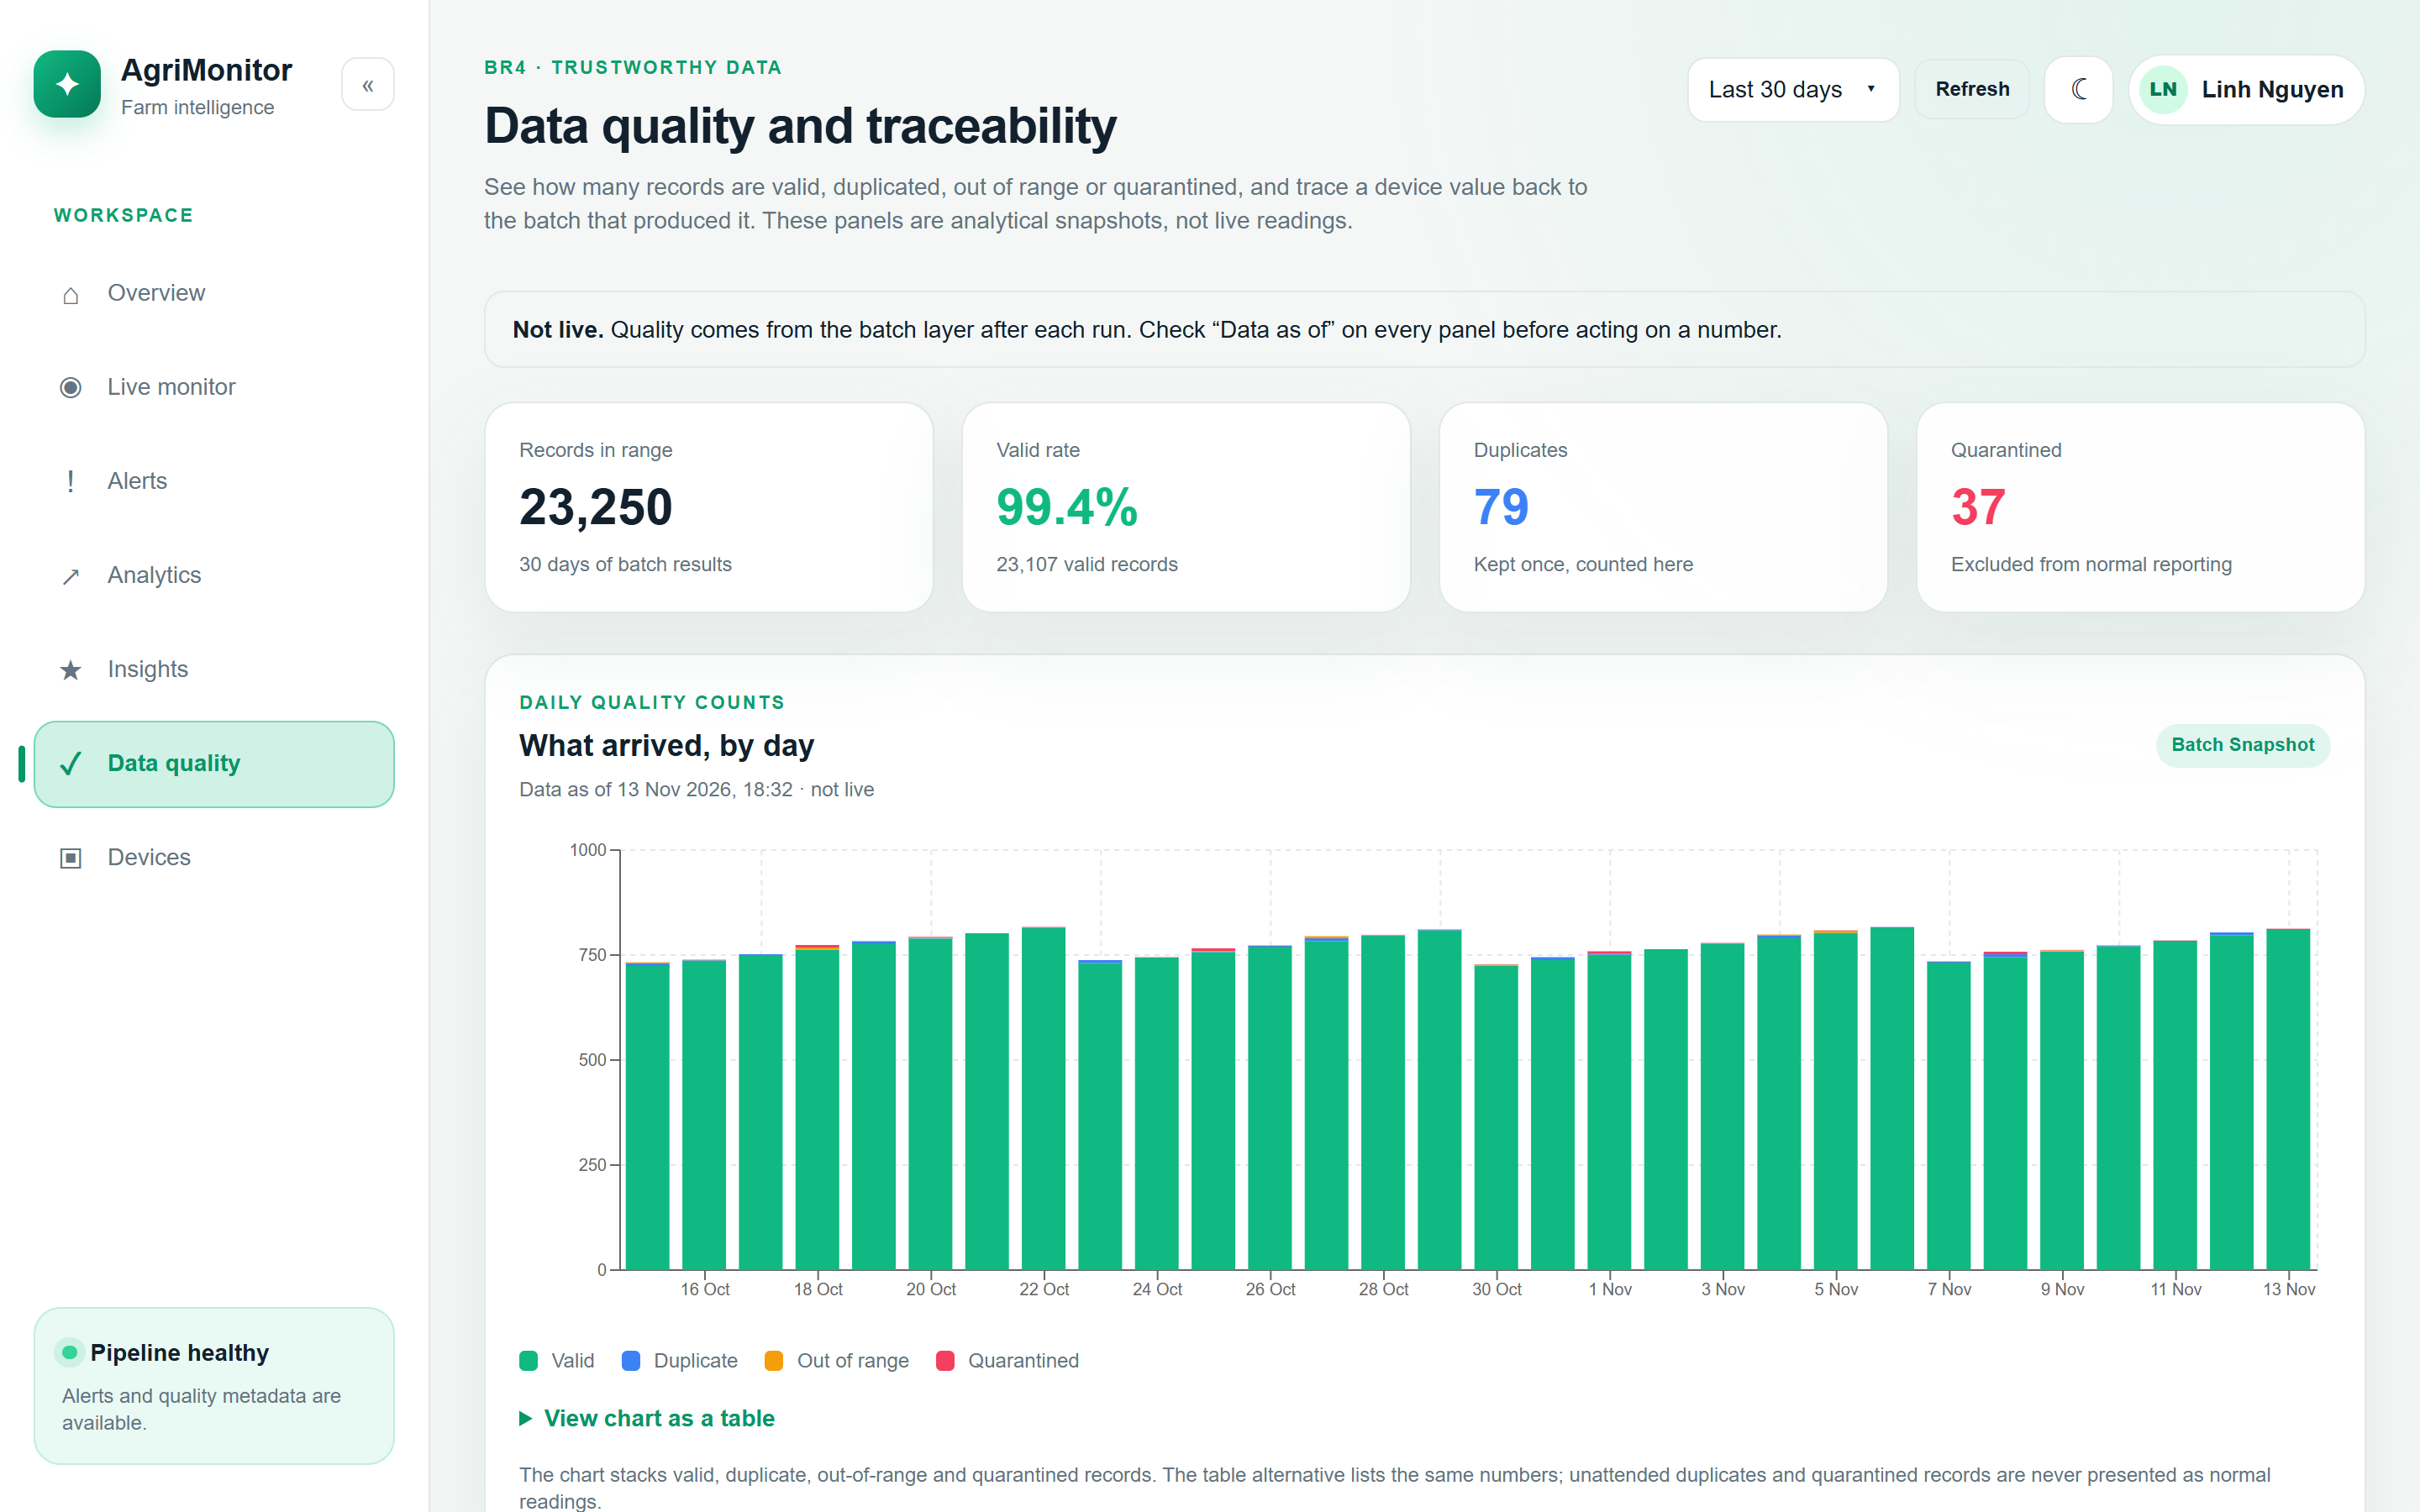
\includegraphics[width=\linewidth]{img/app/quality-chart.png}
\caption{Biểu đồ số bản ghi theo ngày}
\end{subfigure}\hfill
\begin{subfigure}[t]{0.48\linewidth}
\centering
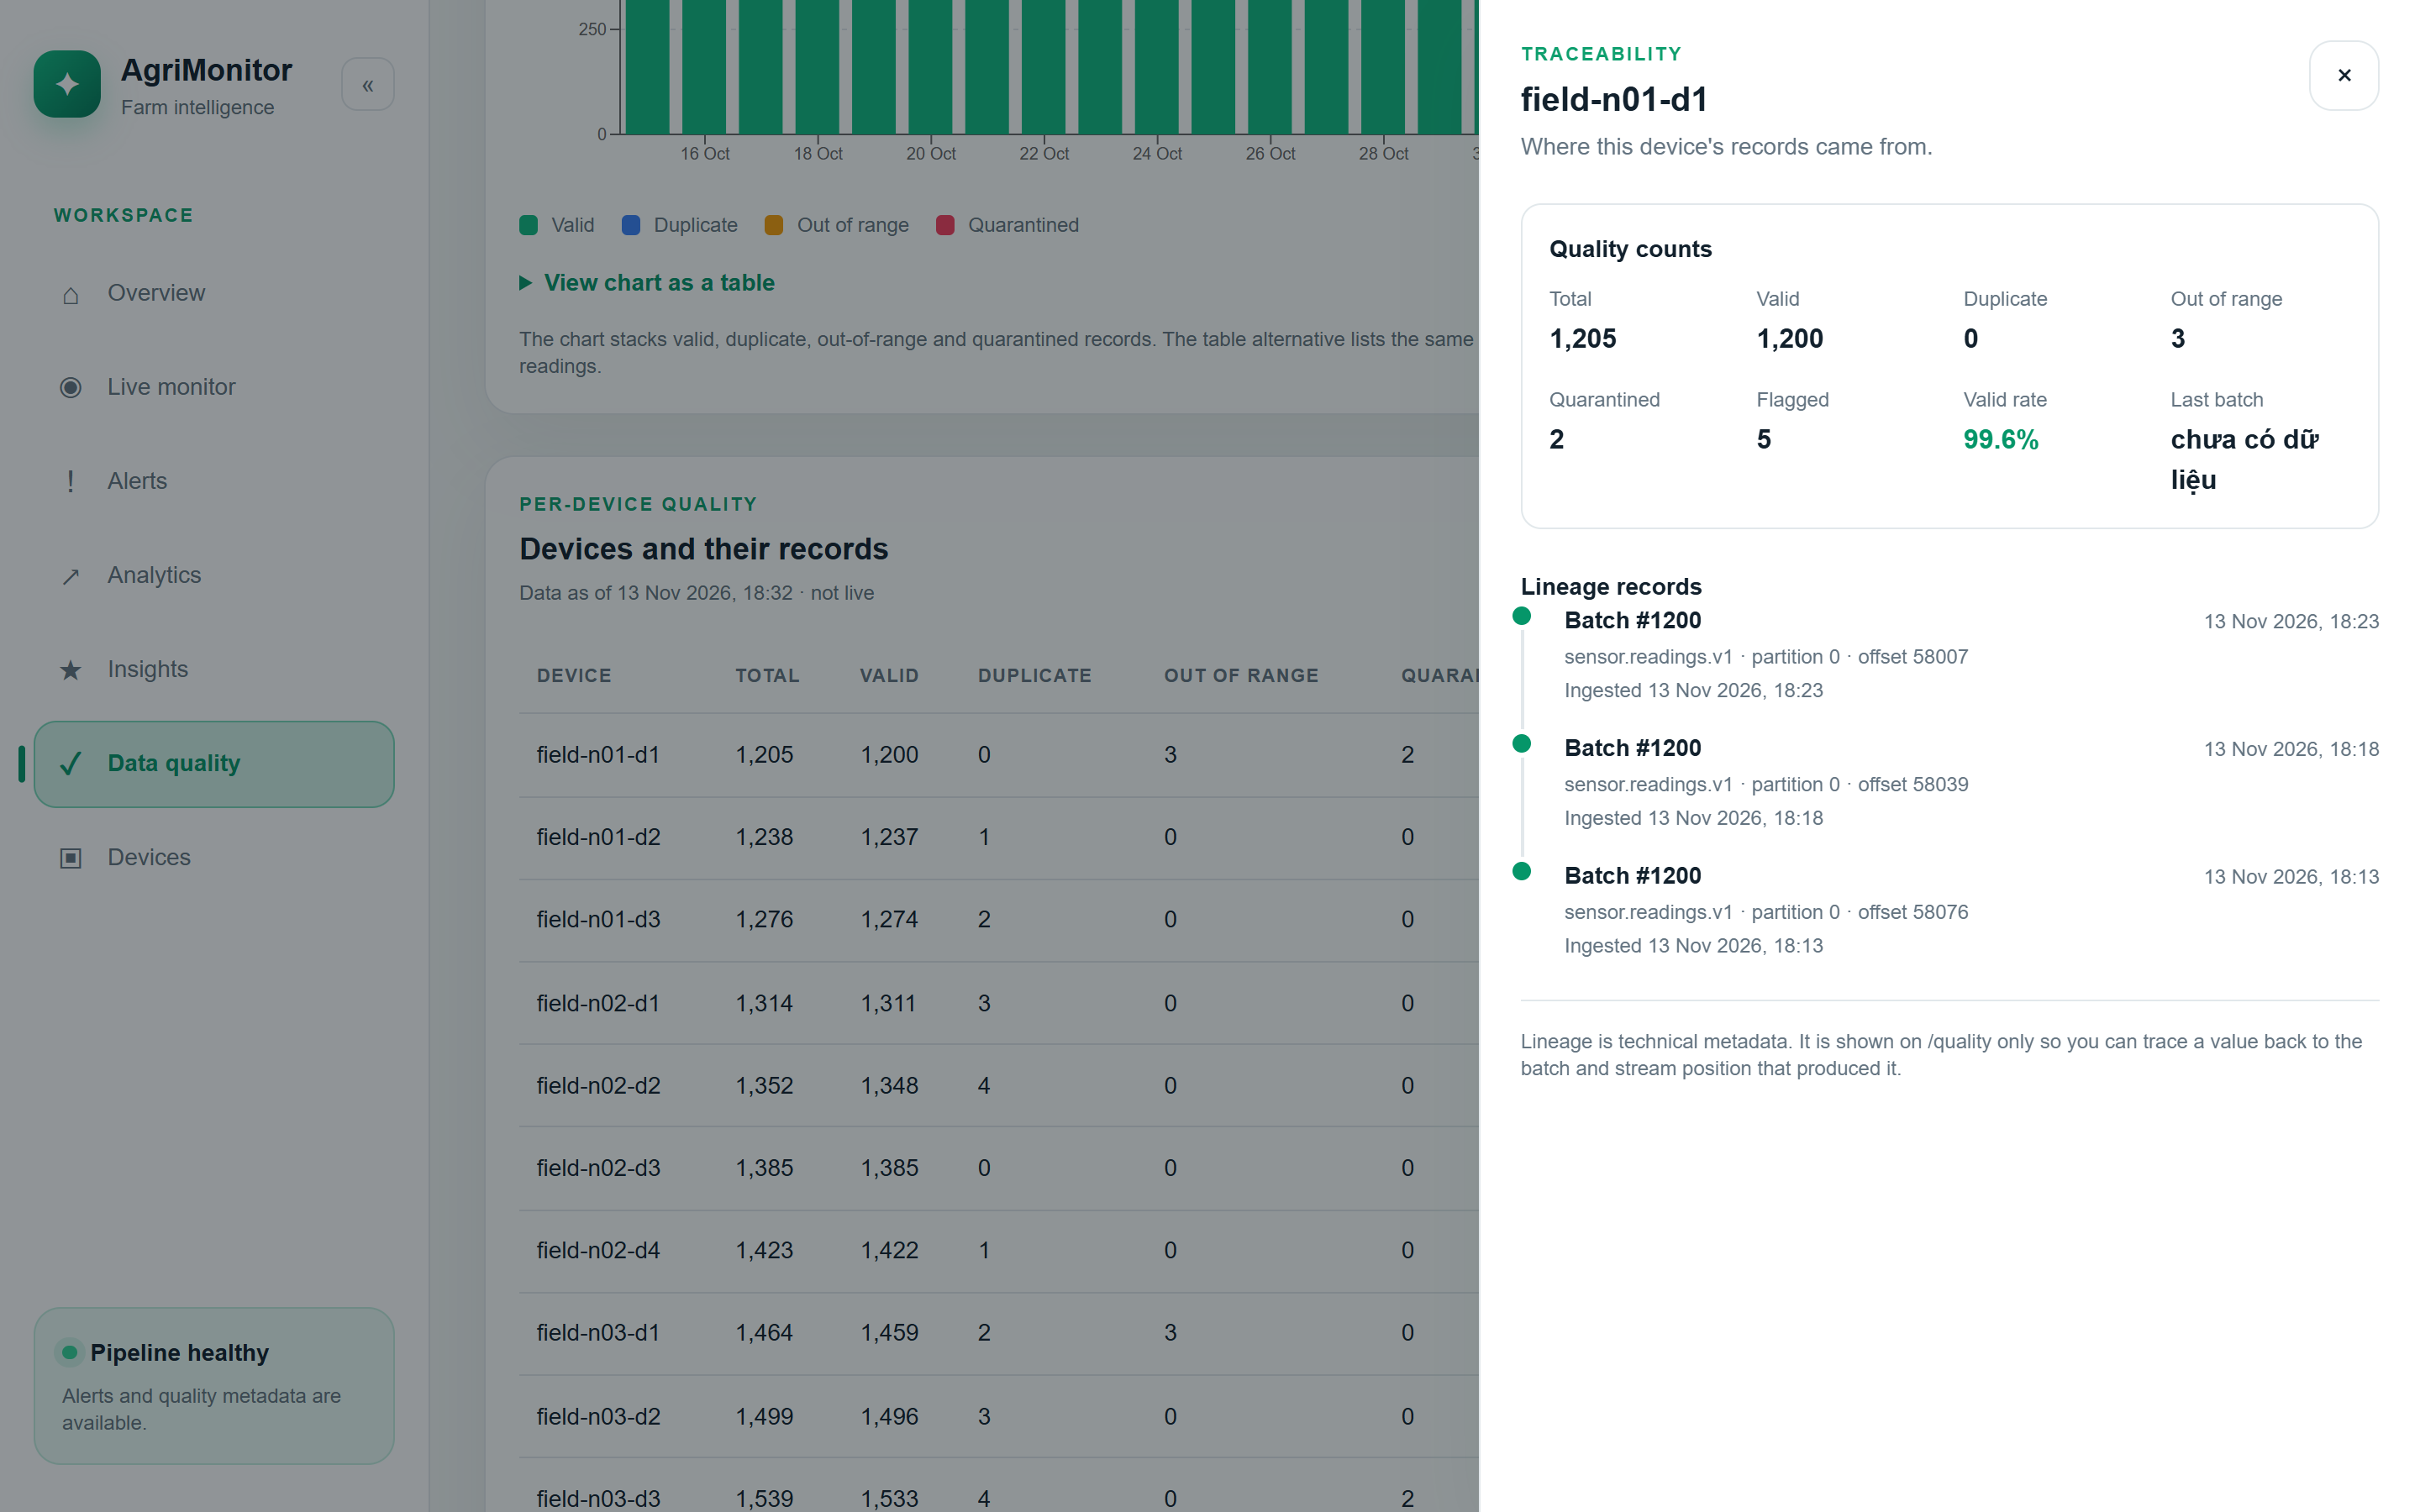
\includegraphics[width=\linewidth]{img/app/quality-lineage.png}
\caption{Lineage của một thiết bị}
\end{subfigure}
\caption{Trang chất lượng dữ liệu của ứng dụng (ảnh chụp với dữ liệu mô phỏng của chế độ \code{DATA\_MODE=mock}).}
\label{fig:4-br04-ui}
\end{figure}

\paragraph{Kết quả và hạn chế hiện tại.} Mọi bản ghi lỗi đều được giữ lại với lý do hoặc cờ, và mọi dòng mang lineage. Có hai điểm còn phải sửa trước khi đánh giá ở Chương~\ref{chap:5-evaluation}. Thứ nhất, model gold \code{field\_daily} hiện tính min, max và trung bình trên mọi giá trị khác rỗng, kể cả dòng có cờ \code{out\_of\_range}; cần giới hạn ở \code{quality\_flag = 'ok'}. Thứ hai, các model gold mới chỉ có test \code{not\_null}; cần thêm test khoảng giá trị (accepted range) để FR4.7 có tác dụng ở tầng gold.
